% !TeX spellcheck = en_US
\documentclass[twocolumn,showpacs,aps,superscriptaddress]{article}
\bibliographystyle{aipnum4-1}

\usepackage{color}
\usepackage{soul}
\definecolor{darkgreen}{rgb}{0,0.6,0}
\definecolor{orange}{rgb}{0.99,0.257,0}
\usepackage{hyperref}
\newcommand{\rot}[1]{{\color{red} #1}}
\newcommand{\ora}[1]{{\color{orange} #1}}
\newcommand{\blau}[1]{{\color{blue} #1}}
\usepackage{graphicx}
\usepackage{amsmath}
\def\mean#1{\langle#1\rangle}
\newcommand{\lr}[1]{\left\langle #1 \right\rangle}
\newcommand{\lrabs}[1]{\left| #1 \right|}
\newcommand{\al}{\alpha}
\newcommand{\bt}{\beta}
\newcommand{\ie}{i.e.\ }
\newcommand{\eg}{e.g.\ }
\newcommand{\eps}{\epsilon}
\newcommand{\epi}{\varepsilon}
\newcommand{\tpr}{t^\prime}
\newcommand{\be}{\begin{equation}}
\newcommand{\ee}{\end{equation}}
\newcommand{\ba}{\begin{eqnarray}}
\newcommand{\ea}{\end{eqnarray}}
\newcommand{\bi}[1]{Fig.~\ref{fig:#1}}
\newcommand{\e}[1]{eq.~(\ref{eq:#1})}
\newcommand{\req}[1]{Eq.~(\ref{eq:#1})}
\newcommand{\lrk}[1]{\left\langle #1 \right\rangle}
\newcommand{\real}[1]{\mathrm{Re}\left(#1\right)}
\newcommand{\imag}[1]{\mathrm{Im}\left(#1\right)}
\newcommand{\uint}[1]{\int\mathrm{d}#1~}
\newcommand{\dint}[3]{\int_{#2}^{#3}\mathrm{d}#1~}
\newcommand{\pint}[1]{\int\mathcal{D}#1~}
\newcommand{\vect}[1]{\boldsymbol{\mathbf{#1}}}
\newcommand{\matr}[1]{\bm{#1}}
\newcommand{\lrexp}[1]{\exp\left(#1\right)}
\DeclareMathOperator\erf{erf}
\DeclareMathOperator\erfc{erfc}
\usepackage{lipsum}

\begin{document}

\title{Critical current for giant Fano factor  in neuron models with bistable firing dynamics and implications for signal transmission}

\author{Richard Kullmann}
\affiliation{Bernstein Center for Computational Neuroscience Berlin, Philippstr.~13, Haus 2, 10115 Berlin, Germany}
\affiliation{Physics Department of Humboldt University Berlin, Newtonstr.~15, 12489 Berlin, Germany}

\author{Benjamin Lindner}
\affiliation{Bernstein Center for Computational Neuroscience Berlin, Philippstr.~13, Haus 2, 10115 Berlin, Germany}
\affiliation{Physics Department of Humboldt University Berlin, Newtonstr.~15, 12489 Berlin, Germany}
\date{\today}

\begin{abstract}
Here the abstract
\end{abstract}	

\maketitle

\section{Introduction}

\section{Noise models: stationary distribution and correlation functions}

\section{Escape out of a cubic potential well}

\section{Summary}
\begin{figure}[h]
\centering
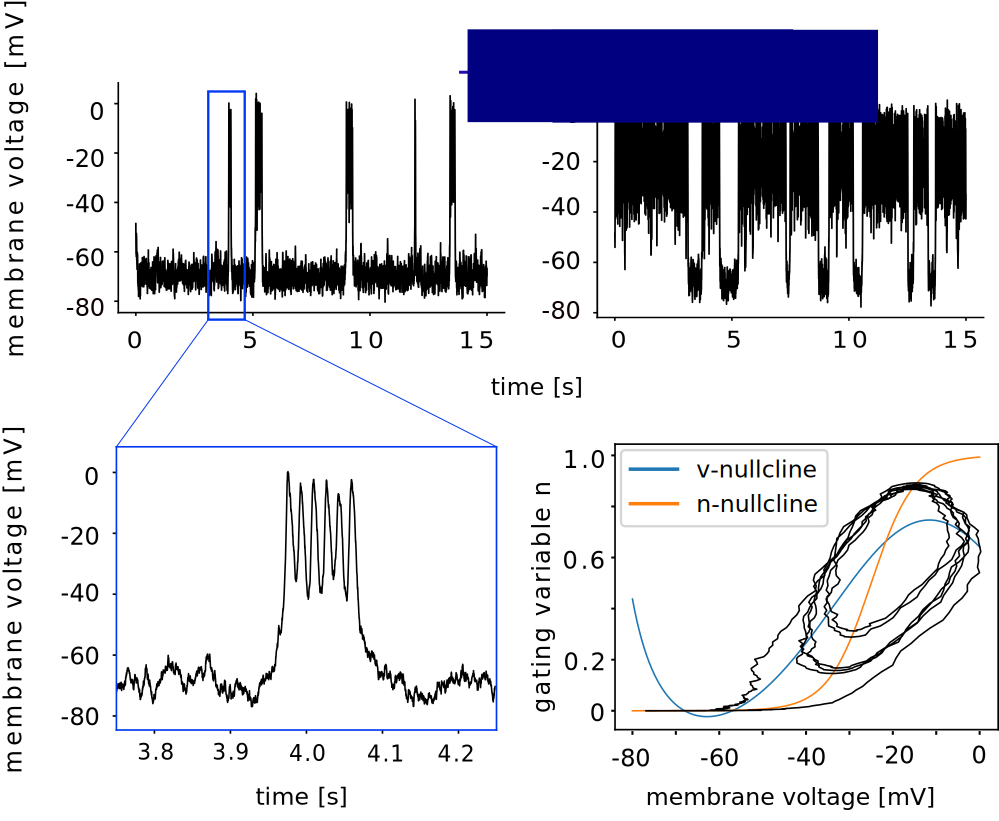
\includegraphics[width=0.45\textwidth]{vtmerge.pdf}
\caption{{\bf A beautiful figure}. Here we give the parameters ...
}
\label{fig:model}
\end{figure}
\section{Summary and conclusions}


\bibliography{ALL_19_03_11}

\end{document}
